% !TEX program = pdflatex
% =============================================================================
%  Peking University -- Technical Report Template
%
%  Compile with pdfLaTeX (REQUIRED). The custom font setup in style.cls relies
%  on pdfTeX's \pdfmapline; xelatex / lualatex will NOT work with this template.
%  In VSCode + LaTeX Workshop the default "latexmk" recipe already uses pdflatex
%  and runs bibtex automatically (a .latexmkrc is included to pin this).
%
%  Placeholder figures use `example-image-duck` from the `mwe` package, which
%  ships with full TeX Live. If you see "File `example-image-duck' not found",
%  install it with:  tlmgr install mwe
% =============================================================================
\documentclass[]{style}

\usepackage[toc,page,header]{appendix}
\usepackage{enumitem}


% For flexible citation formats (author-year, numeric)
\usepackage{natbib}

% For UTF-8 encoded CJK (Chinese, Japanese, Korean) characters
\usepackage{CJKutf8}

% enables \newcommandx
\usepackage{xargs}

% for creating todo notes
\usepackage{todonotes}

% for table \multirow
\usepackage{multirow}


% for \cref
\usepackage{cleveref}

\usepackage{amsmath}
\usepackage{dsfont}

% % using itemize
% \usepackage{enumerate}



% \usepackage{svg}  % needs Inkscape + pdflatex --shell-escape; uncomment only if you use \includesvg

\usepackage{mathrsfs}
\usepackage{adjustbox}
\usepackage{multirow}
\usepackage{multicol}
\usepackage{tcolorbox}
\usepackage{changepage}
\usepackage{enumitem}
\usepackage{graphicx}
\usepackage{amssymb}
\usepackage{xcolor}
\usepackage{float}
\usepackage{multirow}
\usepackage{threeparttable}
\usepackage{graphicx}
\usepackage{subcaption}
\usepackage{algorithm}
\usepackage{algpseudocode}
\usepackage{wrapfig}
\usepackage[table]{xcolor}  % loads xcolor with table support
\usepackage{colortbl}       % gives \columncolor, \rowcolor
\usepackage{tabularx} % Add to your preamble
\usepackage{makecell} % Add to your preamble
\usepackage[dvipsnames]{xcolor}

\newcolumntype{g}{>{\columncolor{gray!10}}c} % gray background
\newcommand{\KVSet}{\mathbf{KV}}
\newcommand{\ModelOuput}{\mathbf{X}_{\theta}}
\newcommand{\KVOutput}{\mathbf{kv}}

\definecolor{catgray}{gray}{0.9}
\definecolor{skyblue}{rgb}{0.53,0.81,0.92} % sky blue

% make it look transparent by mixing with white
\colorlet{skyblue!30}{skyblue!30!white} % 30% skyblue, 70% white

\definecolor{customblue}{RGB}{70,130,180}  % This is equivalent to rgb(70,130,180)

\newtcolorbox{evolbox}[2][]{%
  enhanced,
  % colframe=blue!70!black,
  colframe=customblue,
  colback=white,
  coltitle=white,
  rounded corners,
  boxrule=1pt,
  titlerule=0pt,
  toptitle=1mm,
  bottomtitle=1mm,
  fonttitle=\bfseries,
  % title=#3,
  % fontupper=\boxcontentfont\fontsize{10pt}{12pt}\selectfont,
  width=#2\textwidth, % This takes the second parameter as the width fraction
  % Applying the custom font with size
  % left=1mm, % Reduced left padding
  % right=1mm, % Reduced right padding
  % top=1mm, % Reduced top padding
  % bottom=1mm, % Reduced bottom padding
  #1
}
%%%%%%%%%%%%%%%%%%%%%%%%%%%%%%%%%%%%

\usepackage{minitoc}
\usepackage{url}

% cvpr packages
\PassOptionsToPackage{table,xcdraw}{xcolor}
\usepackage{titletoc}
\usepackage{placeins}
% checkmark / cross symbols for tables
\usepackage{pifont}

% \definecolor{cvprblue}{rgb}{0.21,0.49,0.74}
% \usepackage[pagebackref,breaklinks,colorlinks,allcolors=cvprblue]{hyperref}
\definecolor{RowBlue}{HTML}{E9F2FB}
\definecolor{RowRed}{HTML}{F9EAEA}
\definecolor{Top1}{HTML}{50DB4B} % dark green
\definecolor{Top2}{HTML}{A5FFA2} % medium green
\definecolor{Top3}{HTML}{D9FFD9} % light green
\definecolor{Sub1}{HTML}{EAB8B8}
\definecolor{Sub2}{HTML}{E4E4E4}
\newcommand{\cmark}{\textcolor{green!60!black}{\checkmark}}
\newcommand{\xmark}{\textcolor{red!70!black}{\ding{55}}}

\newcommand{\reviewnote}[1]{{\textcolor{cyan}{[NOTE: #1]}}}
\newcommand{\myparagraph}[1]{\textbf{#1}\hspace{1.8ex}}

\renewcommand{\emph}[1]{\textit{#1}}

\setlength{\cftbeforesubsecskip}{1.5pt}

%%%%%%%%%%%%%%%%%%%% Title / Authors / Affiliation %%%%%%%%%%%%%%%%%%%%

\title{Beyond OCR: A Survey of Document Intelligence\\from Structured Perception to Multimodal Question Answering}

\author{
  JiaShu Yang\texorpdfstring{$^{1}$}{} \hspace{0.1cm}
  Chi Zhang\texorpdfstring{$^{1}$}{} \hspace{0.1cm}
  Xingyu Qi\texorpdfstring{$^{1}$}{} \hspace{0.1cm}
  Ning Zhang\texorpdfstring{$^{1}$}{} \hspace{0.1cm}
  Jie Wu\texorpdfstring{$^{1}$}{} \hspace{0.1cm}
  Lingxu Chen\texorpdfstring{$^{1}$}{} \hspace{0.1cm}
  Jiani Guo\texorpdfstring{$^{1}$}{}
}

% Optional group / team line rendered below the author names, in the same font.
\makeatletter
\g@addto@macro\authorlist{\\[3mm]
  {\authorfont\sffamily Document Intelligence Research Group\texorpdfstring{$^{}$}{}}%
}
\makeatother

\affiliation[]{Peking University}

%%%%%%%%%%%%%%%%%%%% Helper macros (optional, kept from the template) %%%%%%%%%%%%%%%%%%%%
\newcommand{\placeholder}[2]{%
  \fbox{\parbox[c][#1][c]{0.96\linewidth}{\centering\textit{#2}}}}
\newcommand{\answerYes}[1][]{\textcolor{blue}{[Yes]#1}}
\newcommand{\answerNo}[1][]{\textcolor{orange}{[No]#1}}
\newcommand{\answerNA}[1][]{\textcolor{gray}{[N/A]#1}}
\newcommand{\answerTODO}[1][]{\textcolor{red}{\bfseries [TODO]}}
\newcommand{\justificationTODO}[1][]{\textcolor{red}{\bfseries [TODO]}}


\abstract{%
Documents (paper media, images, or electronic files containing textual and graphical information) are ubiquitous in daily office work, online dissemination, and governmental and enterprise workflows; automatically parsing, retrieving, and supporting decision-making based on their content constitutes a core requirement of Document Intelligence. In real-world settings, many documents are first converted into images via scanning or photographing; consequently, document processing typically starts from visual inputs: on the one hand, the system must accurately localize layout elements such as text blocks, tables, figures, and headings, and perform text detection and recognition; on the other hand, it must conduct higher-level semantic understanding and reasoning based on structured inputs to answer queries, extract key information, and generate verifiable results. With advances in deep learning and large language models, the research focus has gradually expanded from ``character-level recognition'' to ``document-level understanding and question answering'' across regions, pages, and modalities, and the field has correspondingly developed evaluation benchmarks that emphasize end-to-end capability and robustness.

Following this evolution, this paper organizes the survey in the order of ``perception first, then reasoning, and finally end-to-end unified modeling,'' and aligns evaluation suites with methodological lineages. Part~I (Document Layout Analysis and OCR) focuses on layout parsing starting from page geometry, including detection/segmentation-based layout element recognition, layout-aware models that incorporate layout information into pretrained representation learning, and robustness and cross-domain generalization under real-world document distributions; it further reviews key technical points of OCR from traditional pipelines to deep learning and lightweight deployment, emphasizing error propagation and engineering constraints when OCR serves as the ``entry point'' for downstream understanding tasks. Part~II (Document Understanding and Question Answering) systematically summarizes three mainstream scenarios built on structured inputs: structure-aware representations for tables, modular/executable reasoning and verifiable question answering; retrieval-augmented generation (RAG) and reasoning-driven retrieval for long texts; and multimodal pretraining and instruction alignment for visually rich documents, along with the evolution toward OCR-free modeling and multi-page, long-context understanding. Finally, we summarize the datasets and benchmarks associated with these two stages, covering task settings from single-page to multi-page documents and from closed sets to real-world enterprise documents, providing reproducible baselines for comparison and a systematic research roadmap for future studies.
}


%%%%%%%%%%%%%%%%%%%% Header links: project page / code / contact %%%%%%%%%%%%%%%%%%%%
\checkdata[
\raisebox{-0.2em}{
\includegraphics[width=0.025\linewidth]{figs/icons/globe.png}}~~Project Page]{\href{https://github.com/your-org/document-intelligence-survey}{\texttt{https://github.com/your-org/document-intelligence-survey}}
\\[-1.5ex]}

\checkdata[
\raisebox{-0.2em}{
\includegraphics[width=0.025\linewidth]{figs/icons/github.png}}~~Code Repository]{\href{https://github.com/your-org/document-intelligence-survey}{\texttt{https://github.com/your-org/document-intelligence-survey}}
\\[-1.7ex]}

\checkdata[
\raisebox{-0.2em}{
\includegraphics[width=0.025\linewidth]{figs/icons/mail.png}}~~Correspondence]{\href{mailto:jiashuyang@pku.edu.cn}{\texttt{jiashuyang@pku.edu.cn}}
\\[-1.7ex]}


\begin{document}
\maketitle


\begin{figure*}[t]
\centering
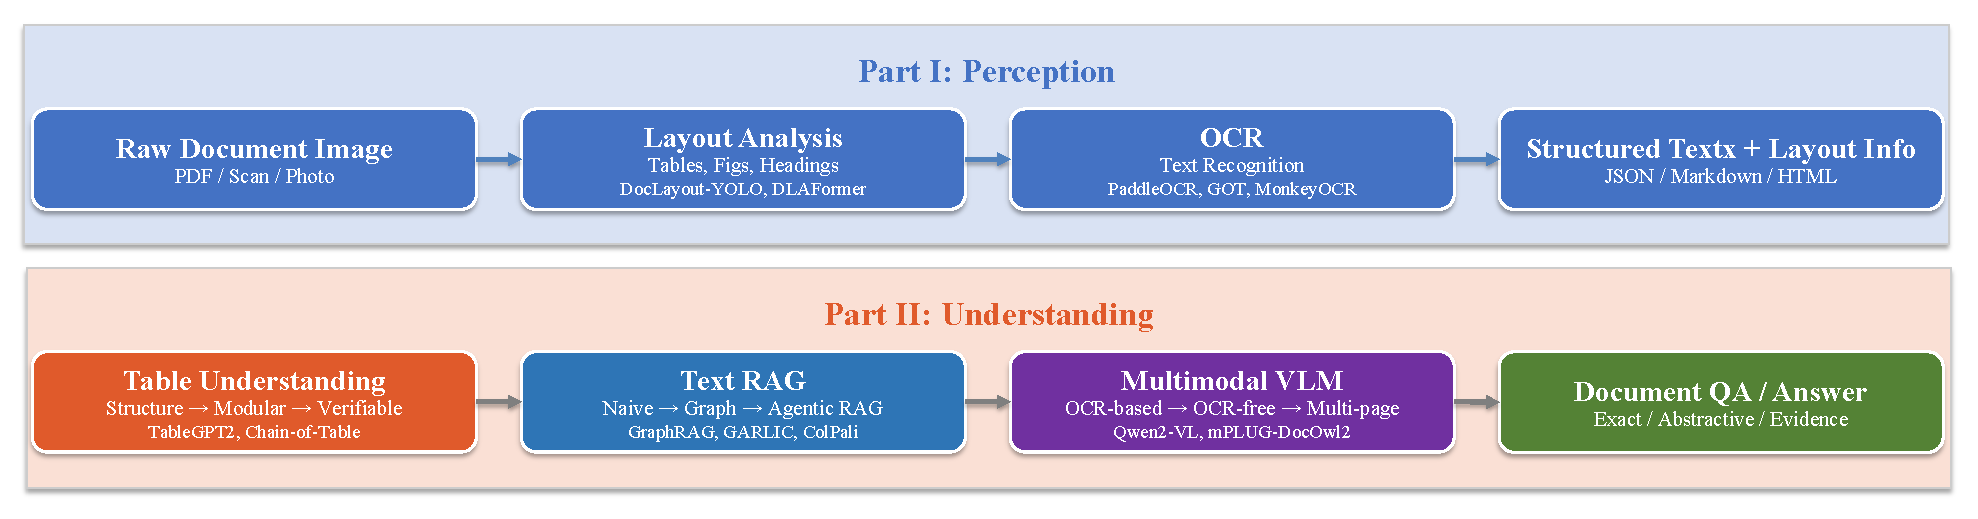
\includegraphics[width=\textwidth]{figs/fig01.pdf}
\caption{Overview of the Document Intelligence pipeline: Part~I (Perception) covers layout analysis and OCR, producing structured text and layout; Part~II (Understanding) includes three parallel branches---table understanding, text RAG, and multimodal VLM---each converging on the final Document QA output.}
\label{fig:pipeline_overview}
\end{figure*}


\section{Introduction}

Documents are fundamental carriers of human knowledge, encompassing a vast array of formats including academic papers, business reports, legal contracts, medical records, and financial statements. The automatic understanding of these documents---extracting structured information, answering questions, and supporting decision-making---has long been a central challenge in artificial intelligence. This field, broadly termed \textbf{Document Intelligence}, has witnessed remarkable evolution over the past decades, driven by advances in computer vision, natural language processing, and more recently, multimodal deep learning.

The document processing pipeline traditionally follows a two-stage paradigm: \textit{perception} followed by \textit{reasoning}. In the perception stage, documents are first converted into machine-readable representations through Optical Character Recognition (OCR) and layout analysis, identifying text regions, tables, figures, and structural elements. The reasoning stage then operates on these structured representations to perform higher-level tasks such as information extraction, question answering, and knowledge synthesis. However, this modular design introduces several challenges: error propagation from OCR to downstream tasks, loss of visual and spatial information during text linearization, and the inability to handle complex layouts that require joint understanding of text, structure, and visual appearance.

With the emergence of large language models (LLMs) and vision-language models (VLMs), the field is undergoing a paradigm shift toward end-to-end, multimodal document understanding. Modern systems can now process document images directly, bypassing explicit OCR stages while achieving superior performance on complex reasoning tasks. This evolution raises fundamental questions: What are the key technical innovations that enabled this transition? How do different approaches---traditional pipelines, retrieval-augmented generation, and unified multimodal models---compare in terms of capabilities and limitations? What evaluation benchmarks best capture real-world deployment requirements?

\subsection{Scope and Contributions}

This survey provides a comprehensive review of document intelligence research, organized around the core pipeline illustrated in \cref{fig:pipeline_overview}. Our contributions are threefold:

\begin{enumerate}[leftmargin=*]
    \item \textbf{Structured Taxonomy}: We present a systematic organization of the field along two dimensions---perception (layout analysis and OCR) and reasoning (table understanding, text-based RAG, and multimodal VLM approaches). This structure reflects the historical evolution while highlighting emerging unified paradigms.
    
    \item \textbf{Technical Depth}: For each research direction, we trace the evolution from early heuristic methods through deep learning innovations to contemporary LLM/VLM-based approaches, emphasizing key architectural decisions, training strategies, and their impact on performance.
    
    \item \textbf{Evaluation Perspective}: We provide a comprehensive overview of benchmarks spanning single-page to multi-page documents, synthetic to real-world distributions, and accuracy-focused to robustness-oriented evaluation protocols, identifying gaps between research metrics and deployment requirements.
\end{enumerate}

\subsection{Organization}

The remainder of this survey is organized as follows. \cref{sec:layout_ocr} covers Part~I: Document Layout Analysis and OCR, including geometric structure detection, layout-aware representation learning, and the evolution of OCR from traditional methods to deep learning and VLM-based approaches. \cref{sec:table,sec:text_rag,sec:vlm} constitute Part~II: Document Understanding and Question Answering, covering table understanding, text-based retrieval-augmented generation, and vision-language models respectively. \cref{sec:eval} reviews evaluation benchmarks and datasets. Finally, \cref{sec:conclusion} discusses future research directions and concludes the survey.

\section{Document Layout Analysis and OCR}
\label{sec:layout_ocr}

This section covers the perception stage of document intelligence, focusing on two fundamental tasks: \textbf{Document Layout Analysis} (identifying and classifying structural elements such as text blocks, tables, and figures) and \textbf{Optical Character Recognition} (converting visual text into machine-readable format). These tasks form the foundation upon which higher-level document understanding is built.

\subsection{Document Layout Analysis}

Document layout analysis has evolved from rule-based heuristic methods to sophisticated deep learning approaches that jointly model visual appearance, textual content, and spatial relationships.

\subsubsection{Geometric Structure Detection and Analysis}

Early approaches treated layout analysis as a computer vision problem focused on detecting and classifying document elements based on their geometric and visual properties. The Document Spectrum method \cite{ogorman1993documentspectrum} characterized page structure from a signal processing perspective, while subsequent work gradually incorporated contextual modeling and detection frameworks.

The deep learning era brought significant advances through the adoption of object detection architectures. Methods such as Faster R-CNN-based approaches \cite{soto2019visual} introduced explicit utilization of contextual information to improve detection robustness in complex layouts. Transformer-based models \cite{yang2022transformerlayout} leveraged global self-attention for document layout understanding, while positional encoding techniques \cite{zhou2022positionalencodinglayout} addressed insufficient modeling of long-range spatial relationships.

Recent research has focused on unifying detection frameworks and improving real-world generalization. The VSR framework \cite{zhang2021vsr} enhanced interaction modeling between layout elements by fusing vision, semantics, and relation modules. Graph-based approaches \cite{wang2023graphicallayout} utilized graph structures to establish global relationships between PDF elements. For cross-domain scenarios, LD-DOC \cite{gao2024lddoc} proposed lightweight domain-adaptive methods, while DocLayout-YOLO \cite{doclayout_yolo_2024} balanced speed and accuracy through synthetic data and global-to-local perception modules.

\subsubsection{Layout-Aware Representation Learning}

Beyond pure visual detection, modern approaches integrate layout information directly into representation learning, enabling models to capture implicit spatial structures and semantic relationships at the representational level.

LayoutLM \cite{xu2019layoutlm} pioneered the joint modeling of text content and 2D positional information within the Transformer pre-training framework, transitioning layout understanding from pure visual parsing to representation learning. Subsequent work addressed various limitations: Position Masking \cite{saha2021position} strengthened positional semantics prediction; LAMPRET \cite{wu2021lampret} introduced visual features through cross-modal contrastive learning; LiLT \cite{wang2022lilt} proposed language-independent layout modeling for cross-lingual robustness.

Recent advances have explored richer spatial relationship modeling. ERNIE-Layout \cite{peng2022ernie_layout} explicitly modeled spatial and structural relationships through layout-knowledge-enhanced pre-training. LayoutMask \cite{tu2023layoutmask} designed differentiated masking strategies for different layout units. Multi-scale Cell-based Layout Representation \cite{shi2023multiscale_cell} proposed cell-level representations fusing word-level and cell-level spatial information. Graph-augmented approaches \cite{arshad2025graph_augmented} introduced graph neural networks to progressively refine fine-grained structural representations.

\subsubsection{Layout-Aware Reasoning and Generation}

As Large Language Models have improved, research has shifted from treating layout as an input feature toward using layout as a reasoning condition and generation target.

DocLLM \cite{wang2024docllm} allowed layout information to directly influence attention calculation by explicitly modeling spatial positions of text blocks. mPLUG-DocOwl 1.5 \cite{hu2024mplugdocowl15} unified document structure modeling from a visual perspective without relying on OCR. LayoutLLM \cite{luo2024layoutllm} enabled active consideration of layout structure during generation through layout instruction tuning.

For retrieval scenarios, LAD-RAG \cite{ladrag2025} enabled cross-page retrieval using layout graphs, while SuperRAG \cite{superrag2025} combined layout relations with graph neural networks for multi-hop reasoning. Structured Multimodal RAG \cite{structuredmmrag2025} improved retrieval relevance by utilizing spatial relationships between document blocks.

In the generation direction, LayoutKAG \cite{layoutkag2024} improved layout generation stability by combining layout knowledge with retrieval examples. LayoutCoT \cite{shi2025layoutcot} decomposed layout generation into step-by-step reasoning. These developments mark the transformation of layout from passive input to active model generation target.

\begin{figure*}[t]
\centering
\includegraphics[
    width=0.95\textwidth,
    trim=1.6cm 2.0cm 4.0cm 1.6cm,
    clip
]{figs/fig03.pdf}
\caption{Hierarchical summary of representative methods in Document Layout Analysis and OCR, organized by research category and sub-task.}
\label{fig:layout_pipeline}
\end{figure*}

\subsection{Optical Character Recognition}

OCR technology has undergone a four-stage evolution (\cref{fig:ocr_evolution}): from rule-based traditional methods, through deep learning approaches with CNN-BiLSTM-CTC pipelines, to Layout-Aware OCR with joint structure modeling, and finally to Vision-Language Model-based OCR with end-to-end, multi-task unified frameworks.

\subsubsection{Traditional Matching and Machine Learning Methods}

Early OCR systems relied on handcrafted features and statistical learning. OCRopus \cite{ocropus2008} adopted a hybrid architectural design with rule-based layout analysis and shallow neural networks for text recognition. Statistical learning approaches \cite{tong2014statistical} applied regression models to OCR post-processing, using external corpora and character-level statistical features to optimize recognition results.

Machine learning classifiers such as SVM and Random Forest \cite{kumar2014implementation} significantly improved recognition robustness in complex backgrounds and multi-font scenarios. Domain-specific applications demonstrated practical value in structured information extraction \cite{rajput2016receipt} and cybersecurity \cite{saravanan2019cybersecurity}. Specialized techniques addressed particular challenges: Gaussian Process Upsampling \cite{stefan2010gaussian} for low-resolution documents, reinforcement learning for character segmentation \cite{bae2012multilingual}, and quality assessment frameworks \cite{mcdonald2016rerunning} for historical document digitization.

\subsubsection{Deep Learning Methods}

The deep learning era established the CNN-BiLSTM-CTC architecture as the dominant paradigm. Calamari \cite{wick2018calamari} provided a high-performance open-source toolkit employing CNNs for visual feature extraction, bidirectional LSTMs for sequential dependencies, and CTC loss for end-to-end training.

Subsequent research pursued two directions: higher accuracy and lighter weight. PP-OCR \cite{du2020ppocr} proposed a three-stage optimization strategy achieving an ultra-lightweight 3.5MB model while maintaining high accuracy. Chargrid-OCR \cite{keremberke2021chargrid} introduced instance segmentation to avoid error accumulation in traditional pipelines. Multilingual systems \cite{pham2021multiplexed} processed multiple languages through shared backbones and script-specific adapters.

Recent advances have explored novel architectures. VISTA-OCR \cite{vista_ocr_2024} pioneered generative OCR using diffusion models. GOT (General OCR Theory) \cite{got_ocr_2024} proposed a unified model processing heterogeneous content including text, formulas, tables, and handwriting. TC-OCR \cite{chen2023tcocr} and DocParseNet \cite{liu2023docparsenet} addressed table-specific recognition through end-to-end pipelines integrating structure and content modeling.

\subsubsection{VLM-Based OCR}

The rise of Vision-Language Models has evolved OCR into a multimodal modeling problem fusing visual perception and semantic understanding. Ocean-OCR \cite{ocean_ocr_2024} adopted the BLIP-2 architecture to uniformly handle text detection, recognition, and semantic understanding across over a hundred languages. DeepSeek-OCR \cite{deepseek2025ocr} proposed Contexts Optical Compression to retain key information using minimal visual tokens.

For logical reasoning, DianJin-OCR-R1 \cite{li2025dianjin} proposed a reasoning-and-tool interleaved framework that utilizes the model's own OCR capability, calls expert OCR tools as references, and synthesizes information through reasoning. MonkeyOCR \cite{li2025monkeyocr} introduced the Structure-Recognition-Relation (SRR) triplet paradigm, breaking through the efficiency-precision trade-off. InstructOCR2 \cite{chen2025instructocr2} and PaddleOCR-VL \cite{du2025paddleocrvl} developed ultra-compact vision-language models for efficient document parsing.

\begin{figure*}[t]
\centering
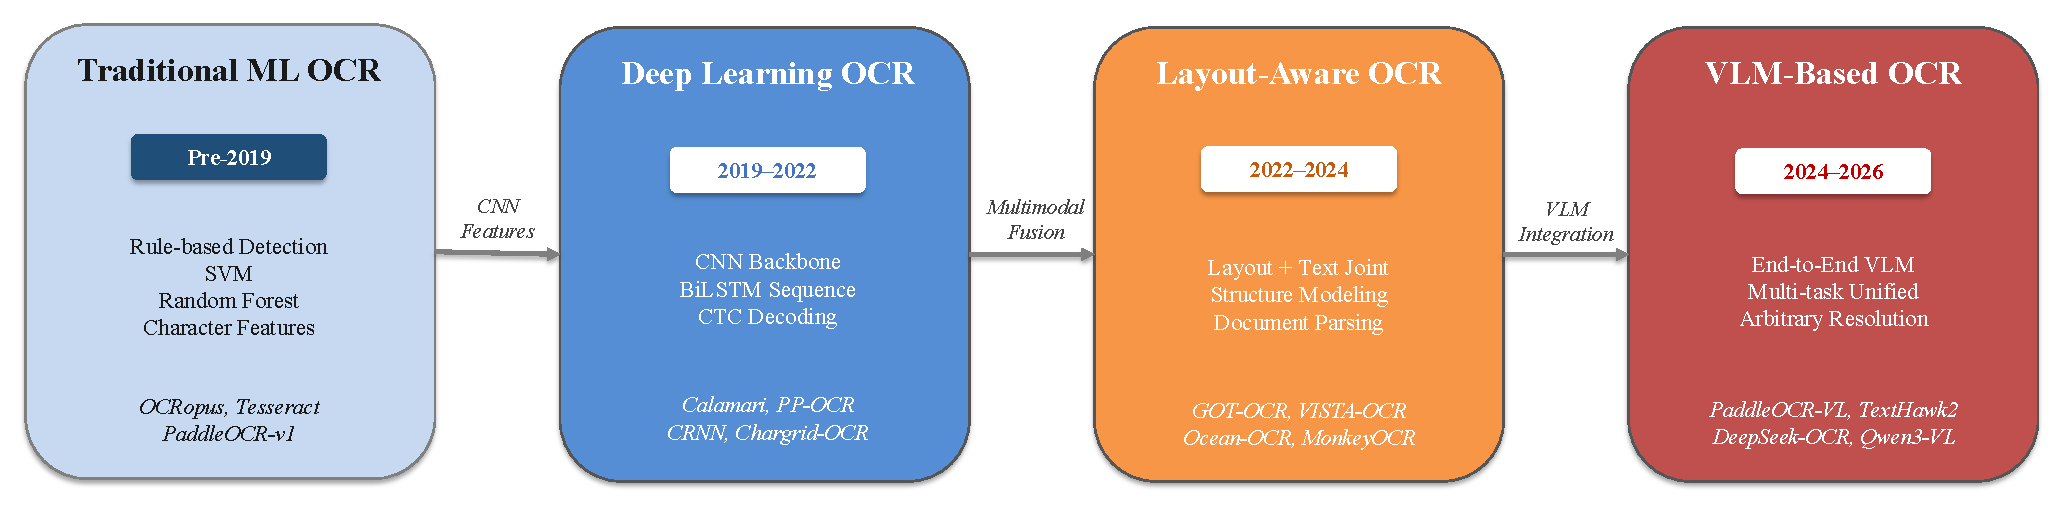
\includegraphics[
    width=0.95\textwidth,
    trim=0cm 0cm 0cm 0cm,
    clip
]{figs/fig02.pdf}
\caption{Four-stage evolution of optical character recognition technology (Pre-2019 to 2024--2026): from rule-based Traditional Machine Learning methods, through Deep Learning approaches with CNN--BiLSTM--CTC pipelines, to Layout-Aware OCR with joint structure modeling, and finally to Vision-Language Model-based OCR with end-to-end, multi-task unified frameworks.}
\label{fig:ocr_evolution}
\end{figure*}

\subsubsection{Layout Analysis and OCR Evaluation}

The evaluation landscape has evolved from task-driven to data-driven approaches. DocVQA \cite{mathew2020docvqa} constructed document visual question-answering tasks through large-scale question-document pairs. PubLayNet \cite{zhong2019publaynet} achieved layout annotation for over 360,000 pages by automatically aligning PDFs and XML files. DocLayNet \cite{pfitzmann2022doclaynet} provided over 80,000 pages of fine-grained human-annotated data from various fields.

For OCR specifically, OCRBench \cite{ocrbench2023} systematically revealed capability boundaries of large multimodal models across 29 sub-tasks. OmniDocBench \cite{omnidocbench2024} built a refined parsing benchmark covering nine document types. Recent datasets address linguistic diversity (SARD \cite{sard2025} for Arabic, 600k-ks-ocr \cite{ksocr2025} for Kashmiri), quality assessment (OCR-Quality \cite{ocrquality2025}), and domain specialization (PubMed-OCR \cite{pubmedocr2025} for scientific literature).

\section{Table Understanding and Question Answering}
\label{sec:table}

Tables present unique challenges for document understanding: they encode structured relational data with implicit row-column dependencies, header hierarchies, and cell-level semantics that are easily lost when linearized into text. This section traces the evolution of table understanding through three stages (\cref{fig:table_stages}): structure-aware representation learning, generation enhancement and modular reasoning, and verifiable reasoning with multimodal understanding.

\subsection{Structure-Aware and Table Semantic Modeling}

Early research recognized that simple table linearization weakened the ability to model row-column relationships and cell dependencies. Work in this stage concentrated on structure-aware representation learning and benchmark construction.

Intermediate pre-training approaches significantly improved table understanding capabilities. Understanding Tables with Intermediate Pre-training \cite{eisenschlos2020understanding} and OmniTab \cite{jiang2022omnitab} introduced large-scale intermediate pre-training and multi-task pre-training to enhance understanding of table structures, numerical relationships, and linguistic alignment. Representations for QA from Documents with Tables and Text \cite{zayats2021representations} and SoarGraph \cite{zhu2023soargraph} emphasized joint modeling of tables and surrounding text, with SoarGraph capturing cross-modal semantic dependencies through graph-structured representations.

Reasoning capabilities were enhanced through specialized pre-training objectives. ReasTAP \cite{liu2023reastap} integrated table reasoning skills during pre-training via synthetic reasoning examples. FORTAP \cite{cheng2022fortap} leveraged spreadsheet formulas for numerical-reasoning-aware table pre-training. At the task level, AIT-QA \cite{katsis2022ait}, FeTaQA \cite{nan2022fetaqa}, and Arxiv Tables \cite{konopka2023arxiv} revealed limitations of traditional methods in complex industry tables, free-form table QA, and long-document table-text associations.

Visual document understanding expanded table research to document images. Visual Understanding of Complex Table Structures \cite{raja2022visual} and HTAN \cite{wu2025htan} proposed robust visual structure modeling for irregular and hierarchical tables. Analytical studies \cite{singha2023tabular,zhao2023large} revealed the sensitivity of LLMs to table representation formats and structural noise, pointing out constraints on their table parsing capabilities.

\subsection{Generation Enhancement and Modular Reasoning}

After establishing fundamental table structure modeling, research shifted toward leveraging LLM generative capabilities through modular, decomposed, and generation-enhanced strategies.

Table instruction tuning emerged as a key paradigm. Table-GPT \cite{peng2023table} performed ``table-tuning'' on general-purpose LLMs using large-scale synthetic table task data. TableGPT2 \cite{su2024tablegpt2} introduced specialized table encoders and multimodal pre-training for complex real-world tables. Rethinking Table Instruction Tuning \cite{deng2025rethinking} systematically analyzed hyperparameter and training scale impacts on performance and generalization.

Modular organization of the generation process enabled more sophisticated reasoning. Localize, Retrieve and Fuse (TAG-QA) \cite{zhao2023localize} supported free-form table QA through a three-stage framework. MFORT-QA \cite{guan2024mfort} combined few-shot learning with multi-hop Chain-of-Thought for cross-table reasoning. Large Language Models are Versatile Decomposers \cite{ye2023large} proposed using LLMs as question and evidence decomposers through a ``decompose-then-reason'' approach.

Input organization and noise suppression techniques improved practical applicability. TACR \cite{wu2024table} utilized table-question alignment for fine-grained cell selection. CABINET \cite{patnaik2024cabinet} reduced interference from irrelevant content through unsupervised relevance scoring. TabSQLify \cite{nahid2024tabsqlify} decomposed large tables into question-relevant sub-tables to reduce context length burdens.

Advanced reasoning methods integrated tables into the reasoning chain. Chain-of-table \cite{zhang2023chainoftable} proposed evolving tables in the reasoning chain. DePlot \cite{liu2023deplot} achieved visual language reasoning through plot-to-table translation. MultiHiertt \cite{wang2023multihiertt} provided numerical reasoning benchmarks for multi-hierarchical tables. Table as Thought \cite{huang2023tableasthought} organized the reasoning process in tabular form to enhance LLM reasoning.

\subsection{Verifiable Reasoning and Multimodal Table Understanding}

Recent research has focused on the verifiability of reasoning processes, execution consistency, and cross-modal reliability to build interpretable and trustworthy table QA systems.

Inference-time scaling and tool integration have improved reasoning capabilities. Table-R1 \cite{yang2025tablegpt1} proposed inference-time scaling for table reasoning through post-training strategies. Weaver \cite{weaver2025} combined SQL with LLMs to dynamically process structured and unstructured data. TableGPT-R1 \cite{yang2025tablegpt} introduced reinforcement learning to mitigate limitations of supervised fine-tuning in multi-step reasoning.

Interpretable reasoning frameworks provide explicit execution trajectories. Interpretable LLM-based Table QA \cite{nguyen2024interpretable} proposed Plan-of-SQLs (POS) to decompose queries into executable SQL sub-steps. Multi-LLM Agent QA over Tabular Data \cite{bangar-etal-2025-exploration} completed planning, code generation, and debugging through multi-agent collaboration.

Tool and execution enhancement approaches strengthen reliability. OpenTab \cite{kong2024opentab} combined table retrieval with SQL execution. TAT-LLM \cite{zhu2024tat} and MATATA \cite{vinayagame2025matata} strengthened discrete and mathematical reasoning through step-wise pipelines. TaPERA \cite{zhao2024tapera} improved trustworthiness through content planning and execution-driven reasoning.

Multimodal table understanding addresses visual table scenarios. TabIQA \cite{nguyen2023tabiqa}, ExpliCIT-QA \cite{hormazabal2025explicit}, and TabPedia \cite{zhao2024tabpedia} emphasized structural recovery, code-interpretable reasoning, and unified multi-task visual table understanding. Knowledge graph integration \cite{raj2024liberating,zhao2025tqagent} reduced hallucinations and supported multi-step tree-like reasoning.

\begin{figure*}[t]
\centering
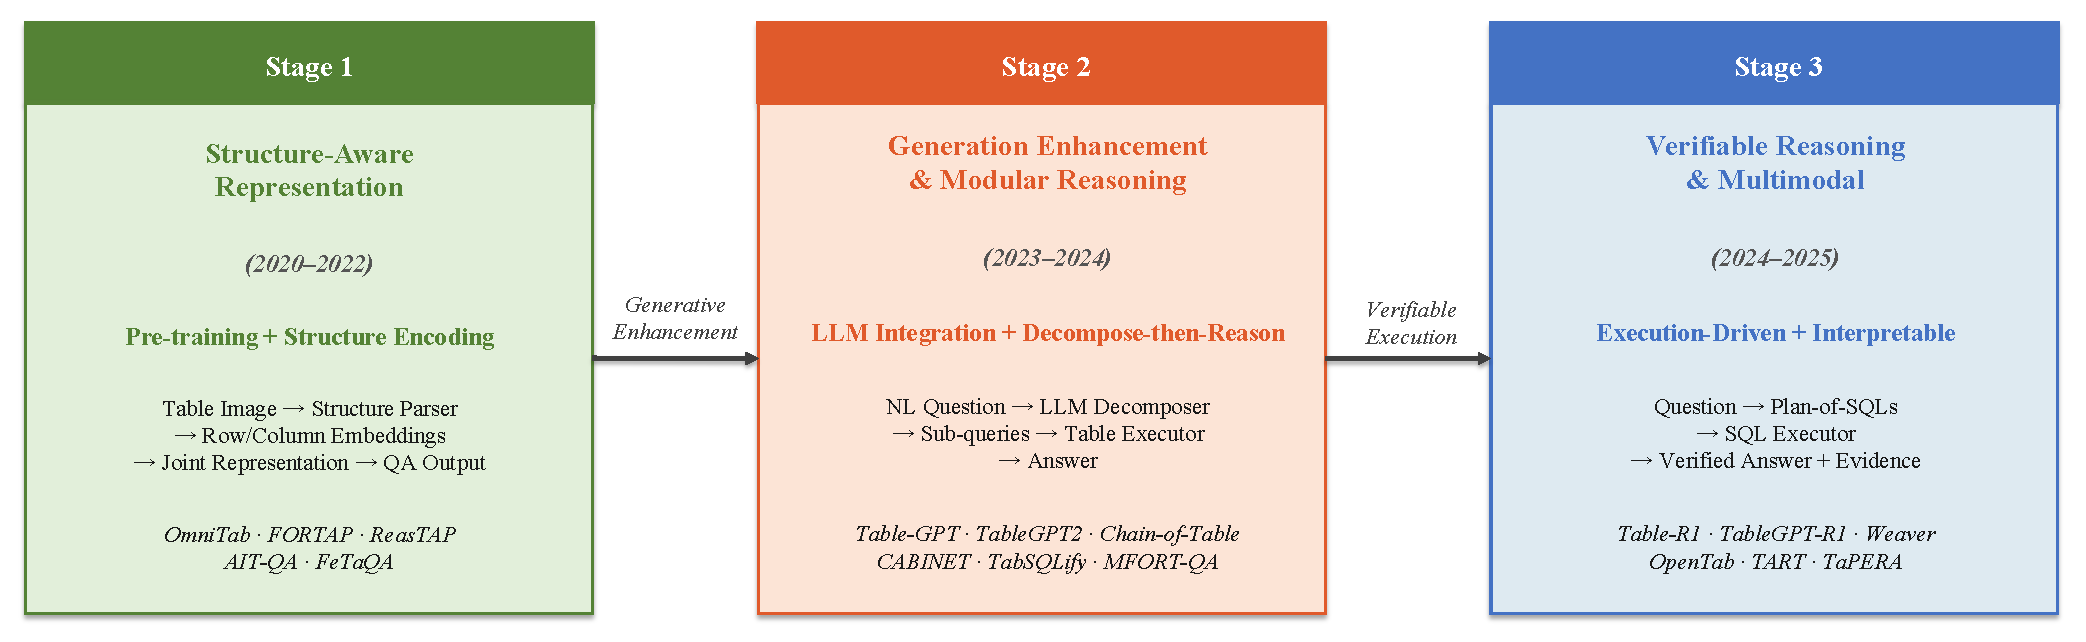
\includegraphics[
    width=0.95\textwidth,
    trim=0cm 0cm 0cm 0cm,
    clip
]{figs/fig05.pdf}
\caption{Three-stage evolution of table understanding and question answering (2020--2025): Stage~1 establishes structure-aware representation learning via pre-training and structure encoding; Stage~2 advances generation enhancement and modular reasoning through LLM integration and decompose-then-reason strategies; Stage~3 achieves verifiable reasoning and multimodal understanding driven by execution and interpretable inference.}
\label{fig:table_stages}
\end{figure*}

\section{Text-Based Retrieval-Augmented Generation}
\label{sec:text_rag}

Document-level question answering faces two core challenges: LLMs are limited by context length for long or multi-document inputs, and pure generative models are prone to hallucinations without external evidence constraints. Retrieval-Augmented Generation (RAG) addresses these challenges by combining information retrieval with text generation. This section traces the five-stage evolution of RAG paradigms (\cref{fig:rag_evolution}): retrieve-then-generate, structure and reasoning-guided RAG, graph-enhanced RAG, multimodal RAG, and agentic RAG.

\subsection{Retrieval-Augmented Generation}

Early RAG followed the classic ``retrieve-then-generate'' paradigm, improving DocQA performance through evidence recall quality and multi-hop support.

Triple-Fact Retriever \cite{wu2022triple} improved cross-document evidence path accuracy by extracting structured triple facts and aggregating evidence hop by hop. Multi-Document Question Answering with Lightweight Embeddings \cite{aitymbetov2024multi} employed two-stage retrieval combining BM25 coarse-ranking with embedding-based re-ranking. Zero-Shot Complex Question-Answering on Long Scientific Documents \cite{wang2025zero} integrated RAG with question decomposition and multi-hop reasoning without task-specific fine-tuning. DR-RAG \cite{hei2024dr} mitigated evidence omission through dynamic document relevance modeling.

\subsection{Structure and Reasoning-Guided RAG}

Subsequent research focused on utilizing LLM reasoning capabilities and document structural information to build structure-aware retrieval frameworks.

DocReLM \cite{wei2024docrelm} fine-tuned retrievers by generating domain-specific training data and citation networks. Advanced Chain-of-Thought Reasoning for Parameter Extraction \cite{chen2025advanced} introduced improved CoT reasoning through targeted document retrieval and iterative optimization. Semi-Structured Chain-of-Thought \cite{su2024semi} unified parametric knowledge, structured knowledge graphs, and unstructured text retrieval.

For long documents, Beyond Chunking \cite{chen2025chunkingdiscourseawarehierarchicalretrieval} utilized Rhetorical Structure Theory for discourse-level modeling and hierarchical retrieval. PdfTriage \cite{saad2024pdftriage} explicitly modeled structural meta-information (pages, sections, tables) for structured long-document QA. Knowledge Graph Prompting for Multi-Document QA \cite{wang2024knowledge} enhanced global consistency through cross-document knowledge graphs.

\subsection{Graph-Enhanced RAG}

Recent research has treated retrieval as a decision-making step directly driven by the reasoning process, utilizing graph structures for evidence organization.

GraphRAG \cite{edge2024graphrag} proposed a graph-enhanced retrieval framework using knowledge graphs and community detection for global, cross-document queries. LightRAG \cite{guo2024lightrag} addressed computational overhead through a lightweight dual-level index architecture. HyperGraphRAG \cite{he2024hypergraphrag} introduced hypergraph structures to model n-ary relations, preserving semantic integrity of complex events.

Dynamic retrieval mechanisms improved evidence continuity. Spreading Activation for Document Retrieval \cite{pavlovic2025leveraging} enabled activation propagation along evidence chains. GARLIC \cite{wang2024garlic} constructed hierarchical weighted graphs for dynamic retrieval path control. HiQA \cite{chen2024hiqa} transformed documents into hierarchical structures with cascading metadata. BookRAG \cite{wang2025bookrag} built BookIndex fusing logical hierarchy trees and entity-relationship graphs.

Multi-hop reasoning was enhanced through iterative expansion. Chain of Retrieval \cite{park2025chain} drove iterative expansion via multi-aspect decomposition and post-order aggregation. Enhancing Document-Level QA via Multi-Hop RAG with LLaMA 3 \cite{huang2025enhancing} integrated dense retrieval, context fusion, and multi-hop mechanisms.

\begin{figure*}[t]
\centering
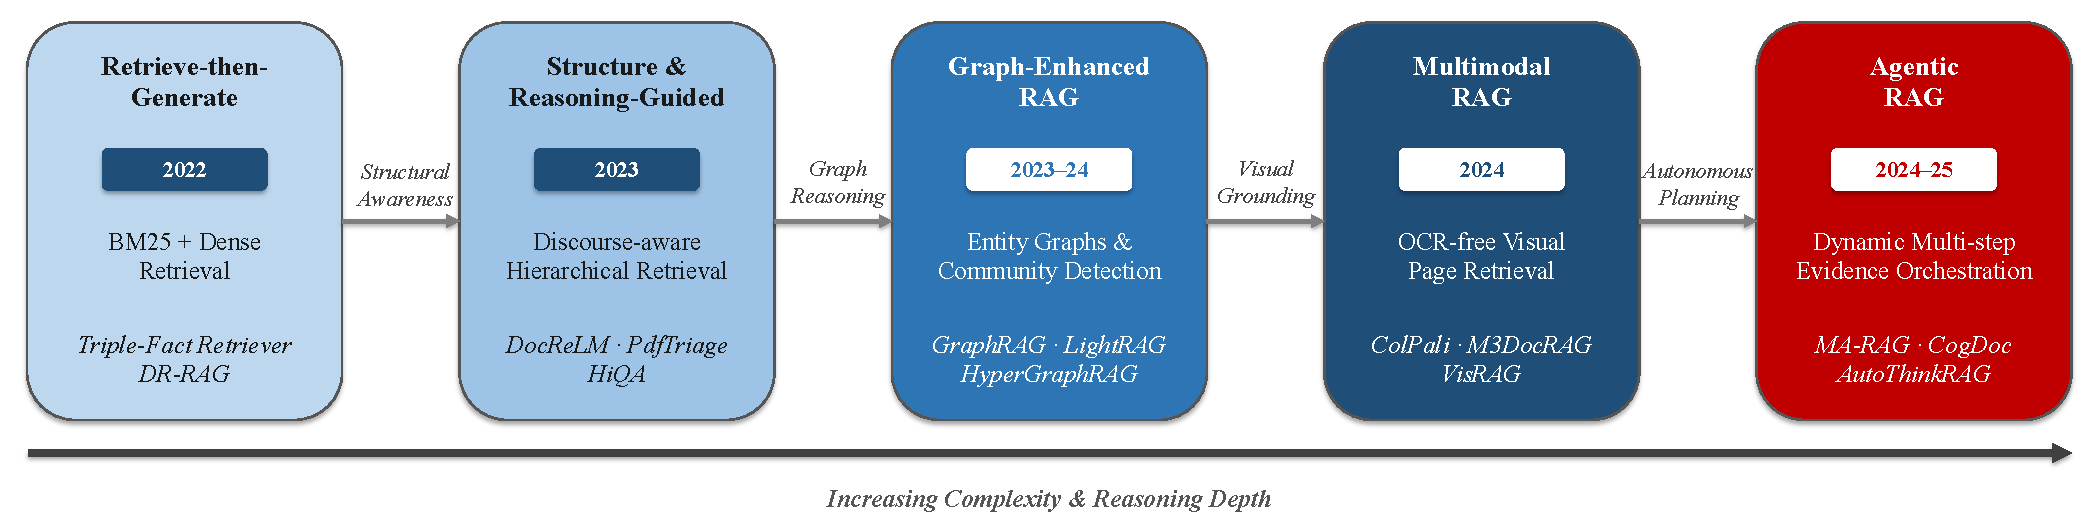
\includegraphics[
    width=0.95\textwidth,
    height=0.38\textheight,
    keepaspectratio,
    trim=0cm 0cm 0cm 0cm,
    clip
]{figs/fig06.pdf}
\caption{Five-stage evolution of retrieval-augmented generation paradigms for document question answering, progressing from Retrieve-then-Generate (2022) through Structure and Reasoning-Guided RAG (2023), Graph-Enhanced RAG (2023--2024), Multimodal RAG (2024), and Agentic RAG (2024--2025), with representative systems listed at each stage and increasing complexity and reasoning depth indicated along the horizontal axis.}
\label{fig:rag_evolution}
\end{figure*}

\subsection{End-to-End Document Question Answering}

Beyond retrieval-augmented approaches, end-to-end document QA has evolved through attention mechanisms, graph-based reasoning, and LLM-era methods.

\subsubsection{Early Attention Mechanisms}

Dynamic Coattention Networks \cite{dynamiccoattention2017} proposed co-attention strategies capturing bidirectional interaction between questions and documents. Coarse-to-fine question answering \cite{coarsetofine2017} pioneered a two-stage framework: first retrieving relevant sentences, then extracting precise answers. EA Reader \cite{eareader2019} utilized multi-space context fusion for improved cloze-style QA.

\subsubsection{Graph Structures and Global Information}

Graph Neural Networks became the core paradigm for connecting discrete evidence. Question Answering by Reasoning Across Documents with GCNs \cite{gcnmultihop2019} utilized entity-based Graph Convolutional Networks for multi-hop tasks. Identifying Supporting Facts with Document Graph Networks \cite{dgn2019} shifted focus to explicit identification of supporting facts through sentence-level document graphs.

Explainable frameworks improved interpretability. Exploiting Explicit Paths \cite{explicitpaths2019} scored and selected evidence paths. Multi-hop Question Answering via Reasoning Chains \cite{reasoningchains2020} used reasoning chains as intermediate explicit variables. Select, Answer and Explain \cite{sae2020} simultaneously generated answers and evidence rationales.

\subsubsection{Task Generalization and the LLM Era}

Multi-hop reasoning expanded to broader tasks. Multi-Hop Transformer \cite{multihoptransformer2021} introduced multi-hop reasoning to translation. Syntax-enhanced multi-hop reasoning \cite{syntaxmultihop2024} advanced document-level relation extraction. MemSum-DQA \cite{memsumdqa2023} streamlined QA model inputs through extractive summarization while preserving evidence integrity.

Recent work explores LLM capabilities for document understanding. Effect of Document Packing \cite{documentpacking2025} examines how document organization affects multi-hop reasoning performance in LLMs.

\section{Vision-Language Models for Document Understanding}
\label{sec:vlm}

Vision-Language Models (VLMs) have propelled visual document understanding from single-modality analysis toward unified multimodal modeling. By jointly modeling visual content, textual semantics, and spatial layout information, VLMs enable deeper understanding of document structures and their semantic relationships. This section traces VLM evolution across four dimensions (\cref{fig:vlm_evolution}): foundational models, high-resolution perception, OCR-free approaches, and agentic systems.

\subsection{Foundational Vision-Language Models}

\subsubsection{Foundational Period of Visually-Rich Document Understanding}

Early research established technical foundations for document image classification and cross-modal retrieval. Deep multimodal learning for cross-modal retrieval \cite{wei2020deep} proposed a ``unified model'' encoding vision and text into the same retrievable representation space.

The pre-training era brought multimodal integration. LayoutXLM \cite{xu2021layoutxlm} introduced multimodal pre-training for multilingual, visually-rich documents. VinVL \cite{zhang2021vinvl} systematically investigated the role of visual features in multimodal tasks. CLIP-Adapter \cite{gao2021clipadapter} proposed efficient adaptation through lightweight feature adapters.

Generalized document processors emerged in 2022. FLAVA \cite{singh2022flava} presented a foundational model using both image-text pairs and unimodal data. UDOP \cite{li2022udop} unified vision, text, and layout as a sequence-to-sequence generative task. Bi-VLDoc \cite{yang2022bivldoc} designed bidirectional vision-language supervision. CM3 \cite{ai2022cm3} adopted causal masked multimodal pre-training for both understanding and generation.

\subsubsection{The Rise of VLM and Advancements in High-Resolution Perception}

LLM integration enabled instruction-driven document understanding. PaLM-E \cite{driess2023palme} proposed an embodied multimodal language model processing various sensor inputs. MiniGPT-4 \cite{zhu2023minigpt4} aligned frozen visual encoders with powerful LLMs through single projection layers. PaLI-X \cite{chen2023palix} scaled multilingual VLMs for document understanding and few-shot learning.

High-resolution processing became a core focus (2023--2024). Monkey \cite{li2024monkey} systematically studied the impact of image resolution and text label quality, noting that resolution improvements often yield more significant gains than structural changes in document scenarios. TextMonkey \cite{li2024textmonkey} proposed an end-to-end OCR-free document understanding model. Qwen2-VL \cite{wang2024qwen2vl} addressed resolution instability through unified modeling supporting arbitrary resolution inputs.

Efficiency and specialization advances included DocKylin \cite{liu2024dockylin} with efficient visual slimming strategies, DocPedia \cite{zhao2023docpedia} exploring frequency-domain information, and Vary \cite{huang2023vary} arguing for visual vocabulary expansion. Small model research \cite{chen2023pali3,li2024slmrvv} achieved strong multimodal understanding at reduced scales.

\begin{figure*}[t]
\centering
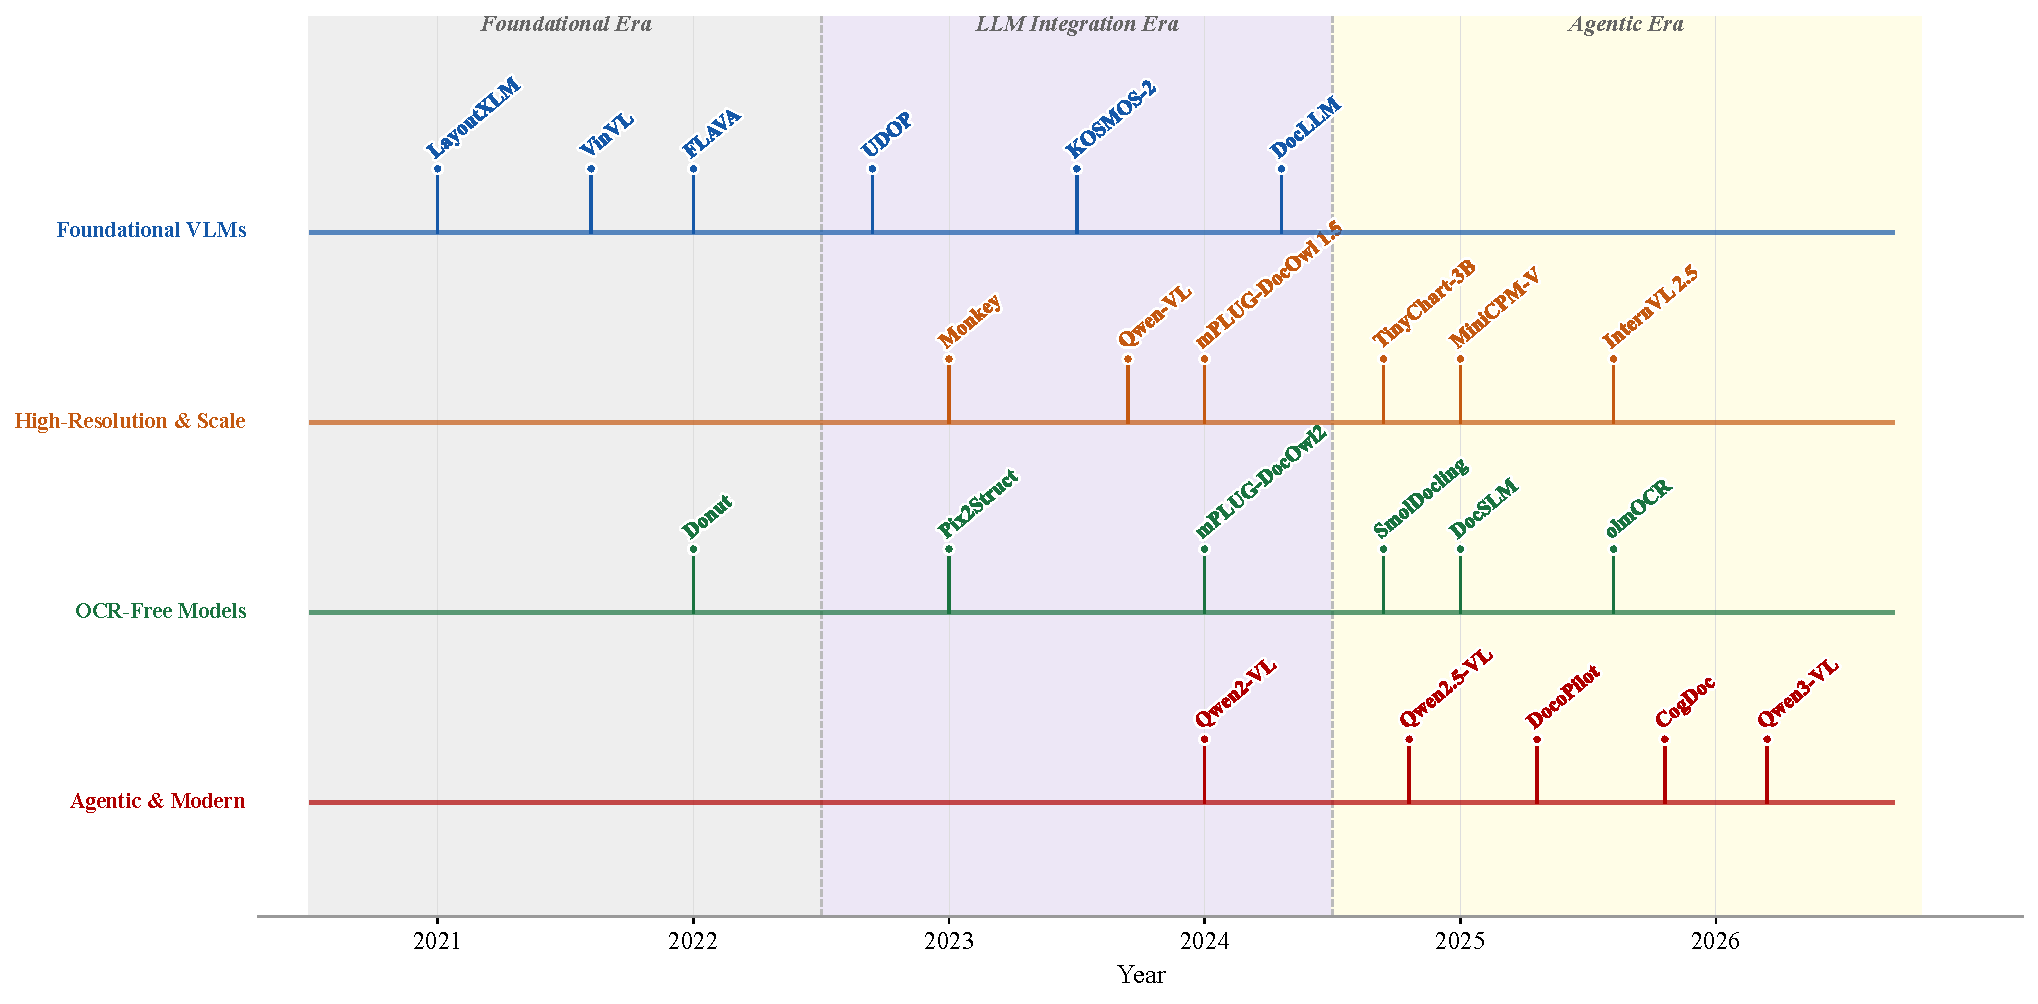
\includegraphics[
    width=0.95\textwidth,
    trim=0cm 0cm 0cm 0cm,
    clip
]{figs/fig07.pdf}
\caption{Evolution of vision-language models for document understanding (2021--2026)---organized into four development tracks: foundational vision-language models, high-resolution and scaled architectures, OCR-free models, and agentic systems for complex document reasoning.}
\label{fig:vlm_evolution}
\end{figure*}

\subsection{OCR-Free and Multi-Page Context}

Traditional document understanding relies on OCR to convert document images into text before semantic analysis, disconnecting ``text recognition'' and ``document understanding'' into independent steps. OCR-free models utilize joint vision-language modeling, taking raw document images as direct input.

Donut \cite{kim2022donut} was an end-to-end document understanding model not relying on OCR systems, generating structured text output directly from raw document images. Pix2Struct \cite{lee2023pix2struct} proposed OCR-free VLM based on screenshot parsing pre-training. mPLUG-DocOwl \cite{ye2023docowl} introduced modularized MLLM for OCR-free document understanding.

Multi-page and long-document capabilities expanded applicability. mPLUG-DocOwl2 \cite{ye2024docowl2} proposed efficient visual compression and structural modeling for multi-page documents. DeepSeek-VL2 \cite{deepseek2024vl2} adopted Mixture-of-Experts architecture for parameter efficiency. PDF-WuKong \cite{li2024pdfwukong} addressed long PDF reading through end-to-end sparse sampling. LongFin \cite{chen2024longfin} introduced models specifically for long financial documents.

Complex document parsing advances included MinerU2.5 \cite{liu2025mineru25} with coarse-to-fine two-stage parsing, and POINTS-Reader \cite{wang2025pointsreader} for distillation-free adaptation. Small VLMs \cite{h2ovl2024mississippi} met privacy-sensitive and on-device scenario needs.

\subsection{Modern Document Understanding Evolution}

The years 2025--2026 witnessed explosive development of ultra-lightweight models. DocSLM \cite{wang2025docslm} addressed computational and memory bottlenecks in long document understanding. SmolDocling \cite{kim2025smoldocling} focused on end-to-end multimodal document conversion through universal DocTags format.

Domain-specific applications expanded. Baseer \cite{albaseer2025baseer} designed specialized VLM for Arabic document OCR. IndoColSmol \cite{rahman2025indocolsmol} targeted multimodal Indonesian document search. Semantic Document Derendering \cite{kim2025derendering} parsed complex documents into editable vector formats.

Document-level strategy research included Docopilot \cite{duan2025docopilot} addressing multi-page document-level tasks, and Nayana \cite{kolavi2025nayana} building multi-task, multimodal, multilingual foundational resources. Qwen2.5-VL \cite{bai2025qwen25vl} and Qwen3-VL \cite{bai2025qwen3vl} established performance benchmarks for unified vision-language understanding.

\subsection{Multimodal RAG}

Building on text RAG success, researchers extended retrieval-augmented paradigms to Visual Document QA, forming early multimodal transitions centered on OCR/structural parsing + text retrieval.

PDF-MVQA \cite{ding2024mvqa} constructed multi-page visually-rich document QA datasets with joint coarse-to-fine retrieval. CREAM \cite{zhang2024cream} introduced coarse-to-fine retrieval pipelines for long contexts. DocLLM \cite{wang2024docllm} mitigated text-layout relationship neglect in traditional VLMs. ViTLP \cite{mao2024visually} jointly modeled text and layout during pre-training.

As ``OCR + text retrieval'' exposed structural and visual information loss, research shifted toward OCR-free visual retrieval. ColPali \cite{faysse2024colpali} proposed page-level OCR-free document retrieval using VLMs for multi-vector page representations, introducing the ViDoRe benchmark. Document Screenshot Embedding \cite{ma2024unifying} used screenshots as unified retrieval input.

Recent multimodal RAG focuses on multi-page, multi-document, multimodal evidence fusion. VisRAG \cite{yu2024visrag} and VDocRAG \cite{tanaka2025vdocrag} pioneered VLM-based retrieval. M3DocRAG \cite{cho2024m3docrag} systematically proposed multi-page, multi-document, multimodal DocQA tasks. CMRAG \cite{chen2025cmrag} mitigated unimodal bias through dual-channel retrieval. RegionRAG \cite{li2025regionrag} lowered retrieval granularity to region level. Luminirag \cite{martis2024luminirag} and MMGraphRAG \cite{wan2025mmgraphrag} unified vision and text into graph structures.

\subsection{Agentic Frameworks for Document QA}

Research has shifted from static RAG to agentic reasoning frameworks with process modeling capabilities.

CuriousLLM \cite{yang2025curiousllm} introduced curiosity-driven follow-up question generation based on Knowledge Graph Prompting, actively guiding retrieval and expanding evidence coverage. DocLens \cite{zhu2025doclens} proposed a tool-enhanced multi-agent framework for long visual document understanding through explicit page-level zooming.

Multi-agent systems improved coordination. MA-RAG \cite{nguyen2025ma} decoupled question decomposition, retrieval control, evidence extraction, and answer synthesis through collaborative chain-of-thought communication. ViDoRAG \cite{wang2025vidorag} proposed dynamic iterative reasoning agents with exploration-reflection workflows.

Research-level complex queries motivated unified systems. Doc-Researcher \cite{dong2025doc} unified multimodal document parsing, dynamic multi-granularity retrieval, and multi-agent reasoning. HEAR \cite{chen2025hear} introduced agentic reasoning into document understanding, establishing coordination between information extraction and reasoning generation. CogDoc \cite{xu2025cogdoc} proposed a unified coarse-to-fine thinking paradigm based on cognitive modeling.

\begin{figure*}[t]
\centering
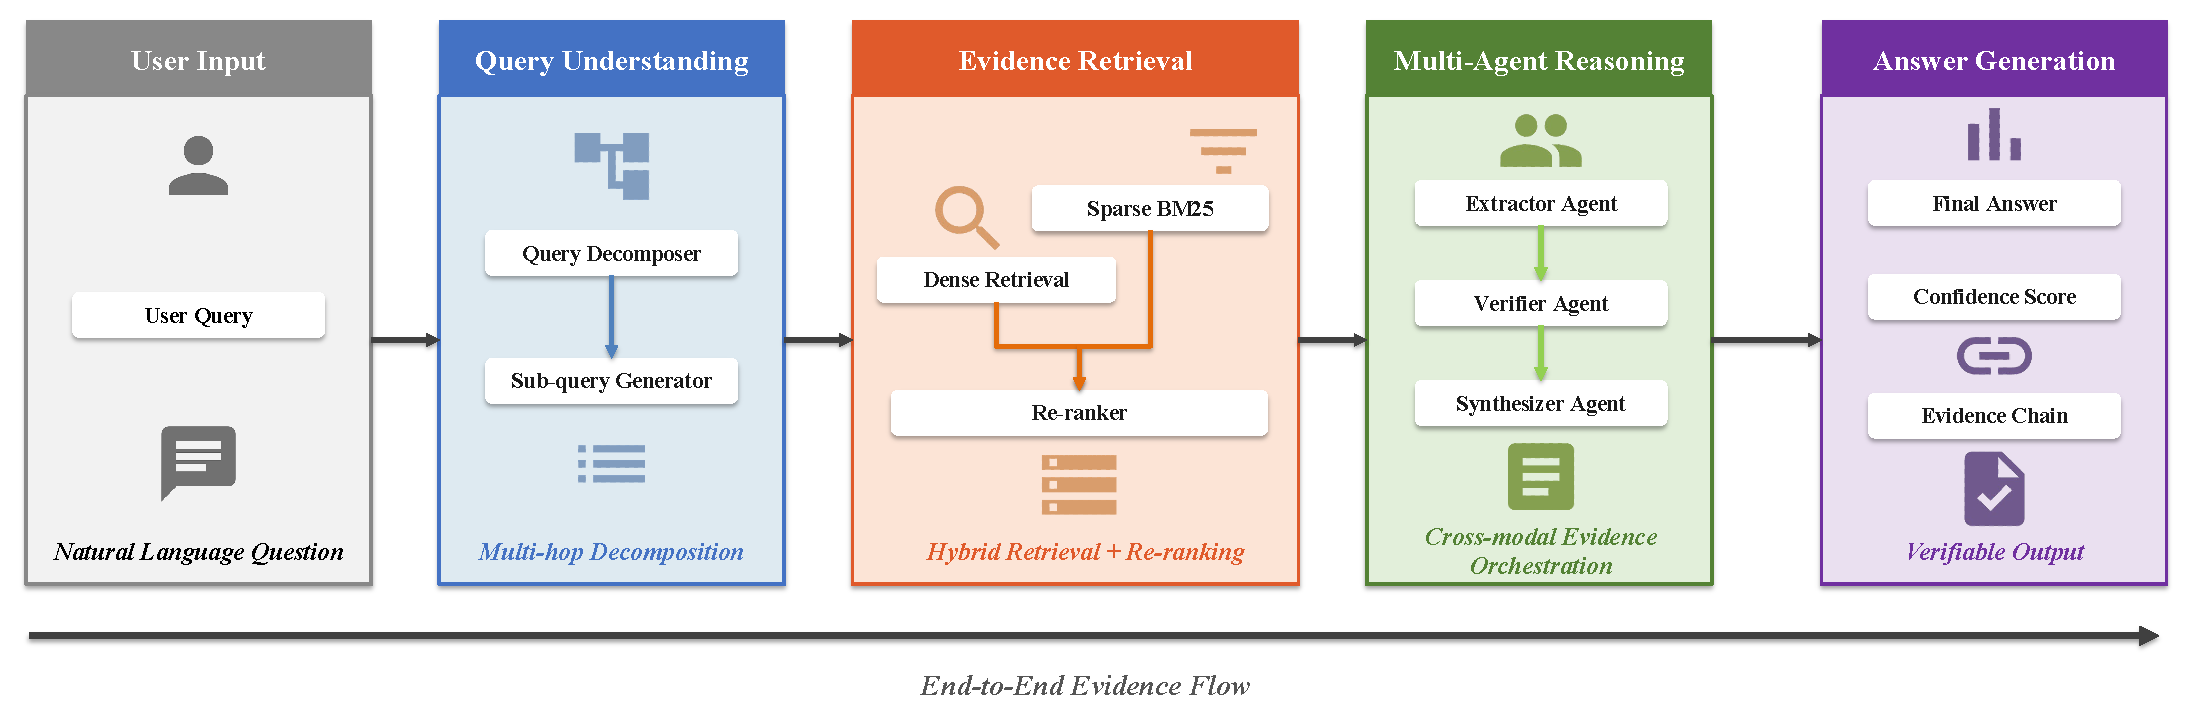
\includegraphics[
    width=0.95\textwidth,
    height=0.40\textheight,
    keepaspectratio,
    trim=0cm 0cm 0cm 0cm,
    clip
]{figs/fig08.pdf}
\caption{Agentic Document QA pipeline illustrating end-to-end evidence flow: a user natural language query passes through Query Understanding (multi-hop decomposition), Evidence Retrieval (hybrid dense and sparse retrieval with re-ranking), Multi-Agent Reasoning (extractor, verifier, and synthesizer agents for cross-modal evidence orchestration), and Answer Generation (producing a final answer with an evidence chain and confidence score).}
\label{fig:agent_docqa}
\end{figure*}

\section{Evaluation}
\label{sec:eval}

With the advancement of Large Language Models, the performance of models in complex document processing and RAG tasks has become a central focus of research. This section reviews evaluation benchmarks spanning visual document understanding, document QA, and real-world image-text interaction scenarios.

\subsection{Visual Document Understanding and Basic QA Evaluation}

Document Question Answering (DocQA) research focuses on whether models can correctly understand text, layout, and visual cues from single-page or small-scale documents.

\subsubsection{Single-Page Document Understanding}

DocVQA \cite{docvqa2020} was among the earliest benchmarks to systematically propose ``question answering on document images,'' emphasizing fact localization through understanding text, layout, and visual cues in single-page documents. Document Collection VQA \cite{doccollectionvqa2021} first placed questions in document collection scenarios, requiring models to locate answers across multiple documents. InfographicVQA \cite{infographicvqa2021} focused on infographic QA to evaluate understanding and reasoning in mixed scenarios of complex layouts, charts, and text.

Scientific and information-seeking benchmarks included A Dataset of Information-Seeking Questions and Answers Anchored in Research Papers \cite{infoseekqa2021}, focusing on question types readers actually ask. DUE \cite{due2021} proposed a comprehensive end-to-end document understanding benchmark where models start from raw documents and complete downstream tasks.

\subsubsection{Cross-Page and Long-Document Understanding}

Research shifted from ``understanding one page'' to ``cross-page understanding and localization.'' Hierarchical Multimodal Transformers for Multi-Page DocVQA \cite{tito2023hierarchicalmultimodaltransformersmultipage} first systematically handled multi-page documents through hierarchical structural modeling. VRDU \cite{vrdu2023} proposed a benchmark specifically for complex business document information extraction. Test-Time Adaptation for Visual Document Understanding \cite{tta-vdu2023} enabled model adaptation at test time.

Datasets with ``locating evidence from many pages'' problem settings emerged. PDFVQA \cite{pdfvqa2023} introduced real PDF documents where questions require locating key information among many pages. SlideVQA \cite{slidevqa2023} studied understanding and reasoning across multiple slide pages. DUDE \cite{dude2023} and DLUE \cite{dlue2023} provided comprehensive evaluation frameworks for visually rich and long complex-structured documents.

Specialized benchmarks addressed particular challenges. KNVQA \cite{knvqa2023} assessed ``factuality'' and knowledge reasoning abilities of Large Vision-Language Models. Privacy-Aware Document VQA \cite{privacydocvqa2023} studied automatic QA under Federated Learning and Differential Privacy constraints. PDFTriage \cite{saad2024pdftriage} evaluated QA capabilities in ``whole book / ultra-long context'' scenarios, emphasizing document structure roles in retrieval and answering.

\begin{figure*}[t]
\centering
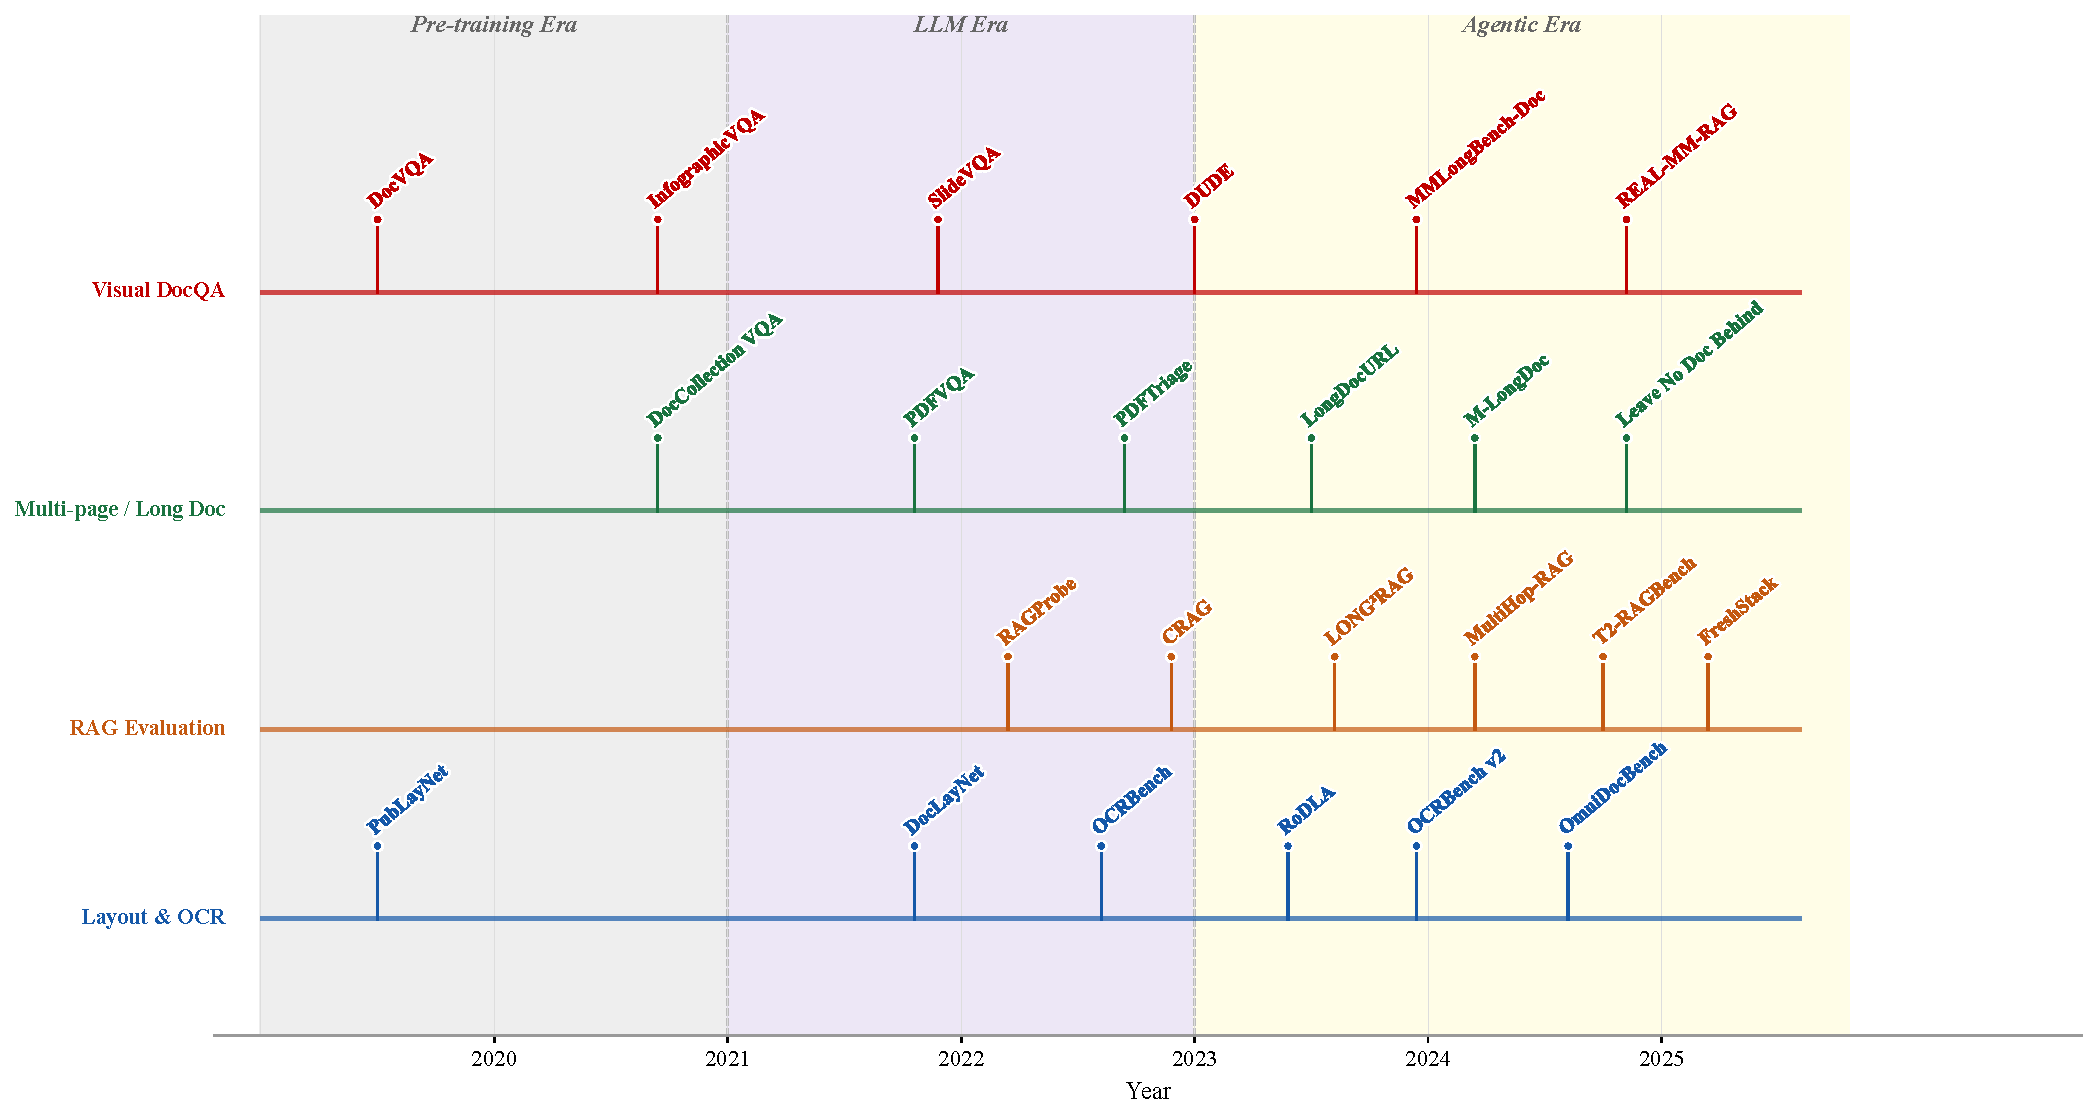
\includegraphics[
    width=0.95\textwidth,
    trim=0cm 0cm 0cm 0cm,
    clip
]{figs/fig10.pdf}
\caption{Benchmark landscape for document intelligence (2019--2025): evaluation datasets are organized into four categories---visual document question answering, multi-page and long-document understanding, retrieval-augmented generation evaluation, and layout analysis with optical character recognition---arranged chronologically by year of publication.}
\label{fig:benchmarks}
\end{figure*}

\subsection{Document QA and RAG Evaluation}

RAG-oriented evaluation explored complex question forms and systematic evaluation frameworks.

\subsubsection{General RAG Evaluation}

RAGProbe \cite{ragprobe2023} evaluated Retrieval-Augmented Generation covering complex question forms in real products (multiple sub-questions, cross-document, unanswerable). CRAG \cite{crag2024} designed task sets covering multiple domains, document structures, and question types for reproducible RAG architecture comparisons.

Explainable and controllable evaluation frameworks emerged. Unanswerability Evaluation for RAG \cite{unanswerablerag2024} measured whether systems correctly refuse unanswerable queries. LONG²RAG \cite{long2rag2024} systematically measured capabilities in ``reading long text, retrieving multiple documents, and generating long answers.'' Fact, Fetch, and Reason \cite{factfetchreason2024} measured end-to-end system performance with multi-hop QA requiring numerical calculation, table queries, and temporal reasoning.

\subsubsection{Domain-Specific and Multilingual Evaluation}

Chinese and domain-specific datasets expanded coverage. CRUD-RAG \cite{crudrag2024} was a large-scale Chinese benchmark abstracting four major application types from ``user interaction with knowledge bases.'' LegalBench-RAG \cite{legalbenchragr2024} measured precision retrieval on complex legal documents. OmniEval \cite{omnieval2024} automatically assessed financial RAG/Agent systems. RAGCare-QA \cite{ragcareqa2025} provided medical RAG evaluation for theoretical medical knowledge QA. RAGPPI \cite{ragppi2024} evaluated PPI-related biological question answering for drug target discovery.

\subsubsection{Long-Context and Multimodal Benchmarks}

Document and multimodal long-context benchmarks matured rapidly. M3DocVQA \cite{m3docvqa2024} provided open-domain, multi-page, multi-document DocVQA. MMLongBench-Doc \cite{mmlongbenchdoc2024} and MMDocBench \cite{mmdocbench2024} tested LVLMs in real long-document PDF scenarios. DOCBENCH \cite{docbench2024} assessed end-to-end document reading system capabilities. LongDocURL \cite{longdocurl2024} focused on complex PDFs of dozens or hundreds of pages, dividing tasks into Understanding, Reasoning, and Locating. M-Longdoc \cite{mlongdoc2024} evaluated ``multimodal ultra-long document understanding'' on hundreds of pages.

\subsection{Real-World Image-Text Interaction Document Evaluation}

Recent datasets involve image-text interaction for real-world settings.

\subsubsection{Multimodal RAG Evaluation}

REAL-MM-RAG \cite{realmmrag2025} focused on real enterprise/document scenarios, emphasizing ``difficult retrieval and high robustness'' across text, tables, and images. CRAG-MM \cite{cragmm2024} was a comprehensive RAG benchmark for multi-modal, multi-person multi-turn dialogue scenarios, focusing on ``wearable devices + visual QA + retrieval augmentation.'' Visual-RAG \cite{visualrag2025} provided text-to-image RAG benchmarks with visual knowledge-intensive questions.

Seeing Through the MiRAGE \cite{mirage2025} measured factuality and citation quality when retrieving, generating, and citing from multimodal sources. UNIDOC-BENCH \cite{unidocbench2025} extracted pages from real enterprise-level PDFs, annotating text blocks, tables, and images with evidence links. VisR-Bench \cite{visrbench2025} proposed a multi-lingual long-document visual retrieval benchmark focusing on ``retrieving the appropriate page from long multi-page documents and then answering.''

\subsubsection{Multi-Hop and Complex Reasoning}

Multi-hop retrieval and reasoning benchmarks developed. MultiHop-RAG \cite{multihoprag2024} systematically evaluated retrieval and reasoning in complex multi-hop QA. DocHop-QA \cite{dochopqa2025} focused on ``cross-document, multi-structure, multi-step reasoning'' scenarios constructed from scientific PDFs. FanOutQA \cite{fanoutqa2024} focused on ``fan-out'' questions requiring simultaneous information integration across numerous entities and documents. MHTS \cite{mhts2025} systematically controlled reasoning difficulty for finer RAG evaluation.

\subsubsection{Structured and Heterogeneous Data}

RAG evaluation on structured heterogeneous data received increasing attention. RAG over Tables \cite{ragovertables2025} provided benchmarks for multi-table QA on large-scale tabular corpora. T2-RAGBench \cite{t2ragbench2025} was a text-table hybrid RAG benchmark for the financial domain. mmRAG \cite{mmrag2025} provided a modular benchmark for heterogeneous/multimodal RAG systems across text, tables, and knowledge graphs.

Dynamic and temporal evaluation emerged. DRAGON \cite{dragon2024} was a dynamic RAG benchmark for news scenarios with continuously changing corpora. FreshStack \cite{freshstack2025} evaluated technical document retrieval in rapidly evolving technical fields.

\subsubsection{Long-Context and Retrieval-Free Control}

Long-context and retrieval-free control evaluations were proposed. LaRA \cite{lara2025} evaluated whether LLMs should rely on ultra-long context or external retrieval. Ko-LongRAG \cite{kolongrag2025} was a Korean long-context RAG benchmark using ``retrieval-free construction.'' Summary of a Haystack \cite{summaryhaystack2024} tested robust long-text understanding in million-token contexts. Are We on the Right Way for Assessing Document RAG? \cite{rightwaydocumentrag2025} analyzed deficiencies of current benchmarks and proposed Double-Bench as an alternative.

\subsubsection{Perceptual and Structural Foundations}

Visual document understanding datasets characterized real document complexity at visual, structural, and linguistic levels. RoDLA \cite{rodla2024} systematically evaluated layout detection stability under real interference. U-DIADS-Bib \cite{udiadsbib2024} focused on pixel-level semantic layout segmentation for ancient manuscripts. M6Doc \cite{m6doc2023} emphasized real scenarios, multiple formats, multiple languages, and complex layouts. MosaicDoc \cite{mosaicdoc2025} provided a large-scale Chinese-English bilingual benchmark from newspapers and magazines. HW-MLVQA \cite{hwmlvqa2025} and MTVQA \cite{mtvqa2025} evaluated multilingual handwritten and text-centric visual QA. IconQA \cite{iconqa2024} focused on diagram reasoning with abstract charts and textbook illustrations.

\section{Future Research Directions and Conclusion}
\label{sec:conclusion}

Although document intelligence has evolved from OCR-centered pipeline approaches to end-to-end systems capable of cross-page, multimodal understanding and retrieval-augmented generation, achieving stable deployment in real-world scenarios still faces critical challenges. These challenges lie not only in a model's ability to understand complex documents, but also in system-level evidence organization and reasoning mechanisms, and in risk-oriented evaluation paradigms for real-world deployment. Future research can be advanced along three levels.

\subsection{Verifiable and Structure-Aware Document Understanding}

Current document question answering systems can often produce seemingly plausible answers, yet these answers frequently lack explicit and verifiable evidence. For example, when asked about a key clause in a contract, a system may generate the correct conclusion but fail to indicate on which page or in which table cell the information is located. This phenomenon---``correct answers but opaque evidence''---limits adoption in high-stakes scenarios, because users cannot easily judge whether the model's reasoning process is trustworthy.

Therefore, a key research direction is to jointly model evidence localization and answer generation, so that while producing an answer, the model can explicitly identify the supporting document regions and establish a correspondence between the answer and its evidence, making the reasoning process verifiable rather than merely plausible.

Meanwhile, document understanding is shifting from pipeline methods that rely on explicit text extraction (e.g., OCR) to end-to-end vision-language models that operate directly on visual inputs. Such OCR-free methods can avoid information loss caused by recognition errors, but they also introduce new challenges: these models no longer have explicit textual and structural boundaries, and thus must automatically learn the document organization internally, such as the hierarchical relations between headings and body text, row and column alignments in tables, and semantic associations across fields.

Without such structure awareness, even if a model can recognize local content, it is difficult to perform consistent and reliable reasoning. Future research should develop structure-aware vision-language modeling methods, enabling models not only to ``see'' document content but also to understand how documents are organized, and to perform content recognition, structural inference, and evidence localization within a unified framework.

\subsection{Multimodal RAG and Agentic Systems for Complex Evidence Organization}

As document understanding tasks extend from single pages to long documents and even collections of multiple documents, the system's challenge is no longer merely to find the page that contains the answer, but to integrate information scattered across different locations into a consistent and reliable conclusion. For instance, an answer may partly come from textual descriptions, partly from tabular data, and partly from figures or supplementary notes on later pages.

Although current methods can retrieve relevant content, they often lack effective mechanisms to confirm whether these pieces of information refer to the same entity or are logically consistent, which can lead to incomplete or even contradictory reasoning results. Future research should develop finer-grained retrieval and representation methods that allow models to localize specific regions in documents, establish cross-page and cross-modal associations, and continuously verify consistency among different evidence during reasoning, rather than relying on one-shot retrieval results.

In addition, in real application scenarios, document understanding is typically not accomplished by a single model, but by the collaboration of multiple functional modules---for example, layout parsing to identify document structure, table parsing to extract structured data, retrieval modules to locate relevant content, and rule-based or computational modules to perform precise verification. Compared with a single model, an agentic system that integrates these tools can dynamically choose appropriate processing steps according to task requirements, thereby improving overall capability.

However, this also brings new research challenges, including how to ensure that the model can reliably select and invoke appropriate tools, how to prevent errors from accumulating throughout multi-step processing, and how to explicitly indicate that a reliable conclusion cannot be reached when evidence is insufficient or conflicting, rather than generating a superficially plausible but ungrounded answer.

\subsection{Risk-Oriented Data and Evaluation Paradigms for Real-World Deployment}

Most existing evaluations of document understanding systems are built on well-structured, high-quality benchmark data, such as well-typeset PDFs or form documents with fixed templates. In such environments, models can often achieve high accuracy. However, documents in real business scenarios are usually more complex: scans may be blurry, skewed, or occluded; documents from different sources can vary substantially in format and language; and key information may be scattered across long contexts or even multiple documents.

This gap between training and evaluation environments and real-world conditions leads to models that perform well on benchmarks but exhibit significant performance degradation in practice. Therefore, future evaluations should pay more attention to generalization under real distributions, including robustness to low-quality documents, adaptability to cross-domain documents, and computational efficiency and stability when handling long documents.

Moreover, existing evaluations typically focus only on whether the final answer is correct, but in practical applications an equally important question is whether the answer is grounded in verifiable evidence. For instance, even if a system occasionally produces the correct answer, users may still find it hard to trust the result if the system cannot explain where the evidence comes from.

Therefore, future evaluations should move beyond a single accuracy metric to multi-dimensional metrics that reflect system reliability, such as whether evidence is correctly localized, whether the reasoning process is internally consistent, whether the system can explicitly indicate uncertainty when it fails, and whether errors are diagnosable. Such risk-oriented evaluation paradigms will more accurately reflect a system's trustworthiness in real-world conditions, and will shift research goals from merely improving average accuracy to building document intelligence systems whose behavior is predictable, whose reasoning is verifiable, and whose behavior in real-world deployment is reliable.

\subsection{Conclusion}

This survey has provided a comprehensive review of document intelligence research, tracing the evolution from traditional OCR and layout analysis through deep learning innovations to contemporary multimodal foundation models. We have organized the field along the core pipeline of perception and reasoning, covering document layout analysis, OCR, table understanding, text-based retrieval-augmented generation, and vision-language models for document understanding.

Key trends emerge from this review: (1) the shift from modular pipelines to end-to-end unified models, (2) the increasing importance of structure-aware and verifiable reasoning, (3) the evolution from single-page to multi-page and long-document understanding, and (4) the growing emphasis on real-world robustness and deployment reliability. These trends point toward a future where document intelligence systems are not merely accurate on benchmarks, but trustworthy, interpretable, and reliable in practical applications.

The challenges ahead are substantial, requiring advances in model architectures, training paradigms, evaluation methodologies, and system integration. However, the rapid progress in foundation models, multimodal learning, and agentic systems provides strong foundations for addressing these challenges. We hope this survey serves as a useful resource for researchers and practitioners working to advance the field of document intelligence.



\clearpage

\bibliographystyle{plainnat}
\setlength{\bibhang}{0pt}
\setlength\bibindent{0pt}
\bibliography{main}

% \clearpage
% \beginappendix
% \input{sec/X_appendix}

\end{document}
